\documentclass[11pt]{article}
\newcommand{\numpy}{{\tt numpy}}    % tt font for numpy

\topmargin -.5in
\textheight 9in
\oddsidemargin -.25in
\evensidemargin -.25in

\textwidth 7in
\usepackage[margin=1in]{geometry}
\usepackage{enumitem}
\usepackage{dirtytalk}
\usepackage{upquote,textcomp}
\usepackage{graphicx}
\usepackage{enumitem}
\usepackage{amsmath}
%\usepackage{enumerate}% http://ctan.org/pkg/enumerate
\usepackage{graphicx}
\usepackage{booktabs}
\usepackage{textcomp}
\usepackage{float}
\usepackage{afterpage}
\usepackage{bm}
\usepackage[linesnumbered,ruled]{algorithm2e}
\restylefloat{table}
\usepackage[table]{xcolor}
\usepackage{multirow}
\usepackage{subfig}% http://ctan.org/pkg/subfig
\usepackage{booktabs}% http://ctan.org/pkg/booktabs
\usepackage{dblfloatfix}

\usepackage{hyperref}
\usepackage{array}
\usepackage{lastpage}
\usepackage{lipsum}
\usepackage{fancyhdr}
\usepackage[hmargin=2cm,top=4cm,headheight=65pt,footskip=65pt]{geometry}

\pagestyle{fancy}
\renewcommand{\headrulewidth}{0pt}
% \fancyhead[CE,CO,LE,LO,RE,RO]{} %% clear out all headers
\fancyhead[C]{{
          \begin{tabular}{|r|c|}
        \hline
        Name: & \hspace{5cm} \\
        \hline
        IIT ID Number: & ~ \\
        \hline
        \end{tabular}
        }
}




\usepackage{array}
\newcolumntype{C}[1]{>{\centering\arraybackslash}m{#1}}

\begin{document}

% ========== Edit your name here
\author{Prof. Kai Shu \\*
Due at 2021 Feb. 7th, 11:59 PM}
\title{\textbf{CS 579: Online Social Network Analysis} \\
[0.2em]\Large{}Homework I - Graph Essentials, Data Mining}
\date{\vspace{-2ex}}
\maketitle

% ========== Name and ID box
\begin{picture}(0,-100) % second value controls the spacing between title and first paragraph
    \put(90,150){ % x, y coordinates for Name box 
                  % (larger x is more right and larger y is further up the page)
    \begin{tabular}{|r|c|}
        \hline
        Name: & \hspace{5cm} \\
        \hline
        IIT ID Number: & ~ \\
        \hline
    \end{tabular}
    }
\end{picture}

\noindent
This is an \textit{\textbf{individual}} homework assignment. Please submit a digital copy of this homework to \textbf{Blackboard}. For your solutions, even when not explicitly asked, you are supposed to concisely justify your answers.
\\
\\

% ========== Begin answering questions here
\begin{enumerate}

    \item \textbf{[Graph Algorithms]}
    \begin{enumerate}[label=(\alph*)]
        \item Compute the shortest path between $v_1$ and other nodes using Dijkstra's algorithm for the following graph. \\
        \begin{figure}[H]
        \minipage{0.7\textwidth}
        \centering
        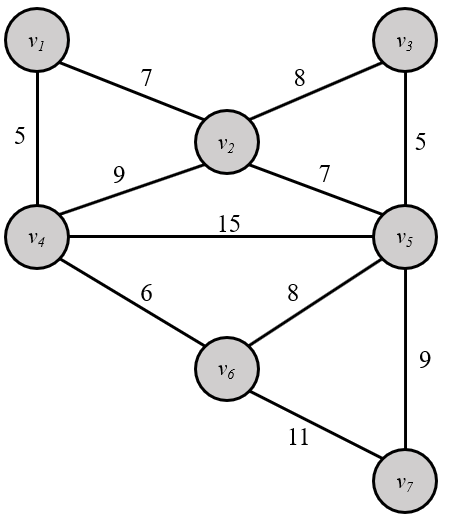
\includegraphics[scale=0.7]{Images/Dijkstra.png}
        \endminipage\hfill
        \minipage{0.3\textwidth}
         \begin{tabular}{ | c | c | } 
         \hline
         \bf Node & \bf Distance from $v_1$\\
         \hline\hline
          $v_2$ & \\
         \hline
          $v_3$ & \\
         \hline
          $v_4$ & \\
         \hline
          $v_5$ & \\
         \hline
          $v_6$ & \\
         \hline
         $v_7$ & \\
         \hline
        \end{tabular}
        \endminipage
        \label{WIS}
        \end{figure}
        
        \newpage
        \item In the space below, draw a simple example of a directed graph with negative-weight edges for which Dijkstra's algorithm produces incorrect answers.\vspace{0.2cm}\\
         \begin{tabular}{ | m{14cm} | } 
         \hline
         \\ \\ \\ \\ \\ \\ \\ \\ \\
         \hline
        \end{tabular} \\
        
        \item Argue whether \say{Algorithm 1} below always produces the shortest paths from one source node to others for graphs that have negative weights but do not have negative cycles.\vspace{0.2cm}
        \\
         \begin{tabular}{ | m{14cm} | } 
         \hline
         \\ \\ \\ \\ \\ \\ \\  \\ \\ \\ \\ \\
         \hline
        \end{tabular}
    \end{enumerate}
    \begin{algorithm}[H]
        \SetKwInOut{Input}{Input}
        \SetKwInOut{Output}{Output}
    
        \Input{Adjacency Matrix $M$, Source node $s$.}
        \Output{Shortest Path from $s$ to other nodes.}
        $C \leftarrow$ Find minimum weight in M\\
        \textbf{for} all $i$ and $j$:\\
              $\qquad M[i,j] \leftarrow M[i,j]-C$ \\
        \textbf{return} Dijkstra(M, s)   $\qquad$ \textit{\small// use the original Dijkstra algorithm to find the shortest paths} 
        \caption{Dijkstra Algorithm for graphs with negative weights.}
    \end{algorithm}
    
    \item \textbf{[Network Algorithms]} For a real-world social network, is BFS or DFS more desirable? Why? Provide details.\vspace{0.2cm}\\
     \begin{tabular}{ | m{15cm} | } 
     \hline
     \\ \\ \\ \\ \\ \\ \\  \\ \\ \\  
     \hline
    \end{tabular}
    \newpage
    \item \textbf{[Decision Tree and Data Types]}
    Consider the given dataset below. Answer the following questions:


    \begin{center}
     \begin{tabular}{|c|c| c| c| c|c|} 
     \hline
     \bf Instance & \bf Age & \bf Income & \bf Student & \bf Credit Rating & \bf Buy Computer \\ [0.5ex] 
     \hline\hline
     1 & 25 & High & No & Fair & No\\ 
     \hline
     2 & 20 & High & No & Excellent & No\\
     \hline
     3 &  32 & High & No & Fair & Yes\\
     \hline
     4 & 45 & Medium & No & Fair & Yes\\
     \hline
     5 & 41 & Low & Yes & Fair & Yes\\  
      \hline
     6 & 41 & Low & Yes & Excellent & No\\  
      \hline
     7 & 36 & Low & Yes & Excellent & Yes\\  
      \hline
     8 & 27 & Medium & No & Fair & No\\ 
      \hline
     9 & 30 & Medium & Yes & Fair & Yes\\ 
      \hline
     10 & 42 & Medium & Yes & Fair & Yes\\ 
     \hline
     11 & 29 & Medium & Yes & Excellent & Yes\\  
      \hline
     12 & 31 & Medium & No & Excellent & Yes\\  
      \hline
     13 & 33 & High & Yes & Fair & Yes\\ 
      \hline
     14 & 41 & Medium & No & Excellent & No\\ 
      \hline
    \end{tabular}
    \end{center}

    \begin{enumerate}[label=(\alph*)]
        \item Specify the data types (Nominal, Ordinal, Interval, Ratio) for each of the four attributes (Age, Income, Student, Credit Rating) in the given data.\\\\
        \newcolumntype{d}{ >{\centering\arraybackslash} m{2.3cm} }
        \begin{tabular}{ | c | d | d | d | c | } 
            \hline
            & \bf Age & \bf Income & \bf Student & \bf Credit Rating \\ [0.5ex] 
            \hline
            \bf Data Type & & & & \\
            \hline
        \end{tabular} \\\\
        
        \item Now assume that we have discretized the real-value \say{Age} attribute into three categories: 1) 30L: \say{Age}$\leq 30$, 2) 41H: \say{Age}$\geq 41$, and 3) BET: $31\leq$\say{Age}$\leq 40$. What is the new data type for the \say{Age} attribute given this change? \\\\
        \begin{tabular}{ | c | d | } 
            \hline
            & \bf Age \\ [0.5ex] 
            \hline
            \bf Data Type & \\
            \hline
        \end{tabular} \\\\
        
        \newpage
        \item Using the ID3 algorithm that we discussed in the class, generate the decision tree for the given dataset. Assume that \say{Buy Computer} attribute is the class
        label and the \say{Age} attribute is discretized as we discussed in previous question. Note that there could be more than one tree that fits the same data and we only need one! Show all your work for each step in making decision tree and explain how you select decision tree nodes and branches.\vspace{0.2cm}\\ 
        \begin{tabular}{ | m{14cm} | } 
        
     \hline
     \\ \\ \\ \\ \\ \\ \\ \\ \\ \\ \\ \\ \\ \\ \\ \\ \\ \\ \\ \\ \\ \\ \\ \\ \\ \\ \\ \\ \\ \\ \\ \\ \\ \\ \\ \\ \\ \\ \\
     \hline
    \end{tabular}
    \end{enumerate}
    
\newpage
    \item \textbf{[Naive Bayes Classification]} 
    Using the Naive Bayes algorithm and the table given in question 3, what would be the label for the following instance.  Assume that “Buy Computer” attribute is the class label and the “Age” attribute is discretized as we discussed in 3.(b).\\\\
    \begin{tabular}{ |c|c| c| c| c|c| } 
            \hline
            & \bf Age & \bf Income & \bf Student & \bf Credit Rating & \bf Buy Computer\\ [0.5ex] 
            \hline
            \bf Instance 15 & 26 & Low & Yes & Fair & ? \\
            \hline
        \end{tabular}\vspace{1cm}\\
        \begin{tabular}{ | m{15cm} | } 
     \hline
     \\ \\ \\ \\ \\ \\ \\  \\ \\ \\  \\ \\ \\  \\ \\ \\  \\ \\ \\  \\ \\ \\
     \hline
    \end{tabular}
\end{enumerate}
\newpage
\begin{tabular}{ | m{15cm} | } 
     \hline
     Notes\\
     \hline
     \\ \\ \\ \\ \\ \\ \\ \\ \\ \\ \\ \\ \\ \\ \\ \\ \\ \\ \\ \\ \\ \\ \\ \\ \\ \\ \\ \\ \\ \\ \\ \\ \\ \\ \\ \\ \\ \\ \\ \\ \\ \\ \\ \\ \\ \\ 
     \hline
    \end{tabular}

\end{document}
\grid
\grid